% Template for PLoS
% Version 3.5 March 2018
%
% % % % % % % % % % % % % % % % % % % % % %
%
% -- IMPORTANT NOTE
%
% This template contains comments intended
% to minimize problems and delays during our production
% process. Please follow the template instructions
% whenever possible.
%
% % % % % % % % % % % % % % % % % % % % % % %
%
% Once your paper is accepted for publication,
% PLEASE REMOVE ALL TRACKED CHANGES in this file
% and leave only the final text of your manuscript.
% PLOS recommends the use of latexdiff to track changes during review, as this will help to maintain a clean tex file.
% Visit https://www.ctan.org/pkg/latexdiff?lang=en for info or contact us at latex@plos.org.
%
%
% There are no restrictions on package use within the LaTeX files except that
% no packages listed in the template may be deleted.
%
% Please do not include colors or graphics in the text.
%
% The manuscript LaTeX source should be contained within a single file (do not use \input, \externaldocument, or similar commands).
%
% % % % % % % % % % % % % % % % % % % % % % %
%
% -- FIGURES AND TABLES
%
% Please include tables/figure captions directly after the paragraph where they are first cited in the text.
%
% DO NOT INCLUDE GRAPHICS IN YOUR MANUSCRIPT
% - Figures should be uploaded separately from your manuscript file.
% - Figures generated using LaTeX should be extracted and removed from the PDF before submission.
% - Figures containing multiple panels/subfigures must be combined into one image file before submission.
% For figure citations, please use "Fig" instead of "Figure".
% See http://journals.plos.org/plosone/s/figures for PLOS figure guidelines.
%
% Tables should be cell-based and may not contain:
% - spacing/line breaks within cells to alter layout or alignment
% - do not nest tabular environments (no tabular environments within tabular environments)
% - no graphics or colored text (cell background color/shading OK)
% See http://journals.plos.org/plosone/s/tables for table guidelines.
%
% For tables that exceed the width of the text column, use the adjustwidth environment as illustrated in the example table in text below.
%
% % % % % % % % % % % % % % % % % % % % % % % %
%
% -- EQUATIONS, MATH SYMBOLS, SUBSCRIPTS, AND SUPERSCRIPTS
%
% IMPORTANT
% Below are a few tips to help format your equations and other special characters according to our specifications. For more tips to help reduce the possibility of formatting errors during conversion, please see our LaTeX guidelines at http://journals.plos.org/plosone/s/latex
%
% For inline equations, please be sure to include all portions of an equation in the math environment.
%
% Do not include text that is not math in the math environment.
%
% Please add line breaks to long display equations when possible in order to fit size of the column.
%
% For inline equations, please do not include punctuation (commas, etc) within the math environment unless this is part of the equation.
%
% When adding superscript or subscripts outside of brackets/braces, please group using {}.
%
% Do not use \cal for caligraphic font.  Instead, use \mathcal{}
%
% % % % % % % % % % % % % % % % % % % % % % % %
%
% Please contact latex@plos.org with any questions.
%
% % % % % % % % % % % % % % % % % % % % % % % %

\documentclass[10pt,letterpaper]{article}
\usepackage[top=0.85in,left=2.75in,footskip=0.75in]{geometry}

% amsmath and amssymb packages, useful for mathematical formulas and symbols
\usepackage{amsmath,amssymb}

% Use adjustwidth environment to exceed column width (see example table in text)
\usepackage{changepage}

% Use Unicode characters when possible
\usepackage[utf8x]{inputenc}

% textcomp package and marvosym package for additional characters
\usepackage{textcomp,marvosym}

% cite package, to clean up citations in the main text. Do not remove.
% \usepackage{cite}

% Use nameref to cite supporting information files (see Supporting Information section for more info)
\usepackage{nameref,hyperref}

% line numbers
\usepackage[right]{lineno}

% ligatures disabled
\usepackage{microtype}
\DisableLigatures[f]{encoding = *, family = * }

% color can be used to apply background shading to table cells only
\usepackage[table]{xcolor}

% array package and thick rules for tables
\usepackage{array}

% create "+" rule type for thick vertical lines
\newcolumntype{+}{!{\vrule width 2pt}}

% create \thickcline for thick horizontal lines of variable length
\newlength\savedwidth
\newcommand\thickcline[1]{%
  \noalign{\global\savedwidth\arrayrulewidth\global\arrayrulewidth 2pt}%
  \cline{#1}%
  \noalign{\vskip\arrayrulewidth}%
  \noalign{\global\arrayrulewidth\savedwidth}%
}

% \thickhline command for thick horizontal lines that span the table
\newcommand\thickhline{\noalign{\global\savedwidth\arrayrulewidth\global\arrayrulewidth 2pt}%
\hline
\noalign{\global\arrayrulewidth\savedwidth}}


% Remove comment for double spacing
%\usepackage{setspace}
%\doublespacing

% Text layout
\raggedright
\setlength{\parindent}{0.5cm}
\textwidth 5.25in
\textheight 8.75in

% Bold the 'Figure #' in the caption and separate it from the title/caption with a period
% Captions will be left justified
\usepackage[aboveskip=1pt,labelfont=bf,labelsep=period,justification=raggedright,singlelinecheck=off]{caption}
\renewcommand{\figurename}{Fig}

% Use the PLoS provided BiBTeX style
% \bibliographystyle{plos2015}

% Remove brackets from numbering in List of References
\makeatletter
\renewcommand{\@biblabel}[1]{\quad#1.}
\makeatother



% Header and Footer with logo
\usepackage{lastpage,fancyhdr,graphicx}
\usepackage{epstopdf}
%\pagestyle{myheadings}
\pagestyle{fancy}
\fancyhf{}
%\setlength{\headheight}{27.023pt}
%\lhead{
\includegraphics[width=2.0in]{PLOS-submission.eps}}
\rfoot{\thepage/\pageref{LastPage}}
\renewcommand{\headrulewidth}{0pt}
\renewcommand{\footrule}{\hrule height 2pt \vspace{2mm}}
\fancyheadoffset[L]{2.25in}
\fancyfootoffset[L]{2.25in}
\lfoot{\today}

%% Include all macros below

\newcommand{\lorem}{{\bf LOREM}}
\newcommand{\ipsum}{{\bf IPSUM}}


\usepackage{booktabs}
\usepackage{longtable}
\usepackage{array}
\usepackage{multirow}
\usepackage{wrapfig}
\usepackage{float}
\usepackage{colortbl}
\usepackage{pdflscape}
\usepackage{tabu}
\usepackage{threeparttable}
\usepackage{threeparttablex}
\usepackage[normalem]{ulem}
\usepackage{makecell}
\usepackage{xcolor}

\usepackage{placeins}



\usepackage{forarray}
\usepackage{xstring}
\newcommand{\getIndex}[2]{
  \ForEach{,}{\IfEq{#1}{\thislevelitem}{\number\thislevelcount\ExitForEach}{}}{#2}
}

\setcounter{secnumdepth}{0}

\newcommand{\getAff}[1]{
  \getIndex{#1}{Pontificia Universidad Católica de Chile}
}

\providecommand{\tightlist}{%
  \setlength{\itemsep}{0pt}\setlength{\parskip}{0pt}}

\begin{document}
\vspace*{0.2in}

% Title must be 250 characters or less.
\begin{flushleft}
{\Large
\textbf\newline{\emph{Delphinidae} whale watching and biodiversity with an emphasis on
\emph{Orcinus Orca}} % Please use "sentence case" for title and headings (capitalize only the first word in a title (or heading), the first word in a subtitle (or subheading), and any proper nouns).
}
\newline
% Insert author names, affiliations and corresponding author email (do not include titles, positions, or degrees).
\\
Esteban Jorquera\textsuperscript{\getAff{Pontificia Universidad Católica de Chile}}\textsuperscript{*}\\
\bigskip
\textbf{\getAff{Pontificia Universidad Católica de Chile}}Pontificia Universidad Católica de Chile, Biological Sciences, Marcoleta
49, Santiago, RM\\
\bigskip
* Corresponding author: eijorquera@uc.cl\\
\end{flushleft}
% Please keep the abstract below 300 words

% Please keep the Author Summary between 150 and 200 words
% Use first person. PLOS ONE authors please skip this step.
% Author Summary not valid for PLOS ONE submissions.

\linenumbers

% Use "Eq" instead of "Equation" for equation citations.
\hypertarget{introduction}{%
\section{Introduction}\label{introduction}}

Observing cetaceans (whales and dolphins) in their natural habitat, by
either observing directly from the coast or going into the open ocean,
is a recreational activity that is quickly gaining popularity and
becoming a booming touristic industry, in what is known as whale
watching {[}1{]}.

The practice originated in the United States during the early fifties
with the observation of the migratory behavior of grey whales near the
Cabrillo National Monument area in San Diego and spread throughout the
Pacific coast of the US. In the Atlantic coast, the Montreal Zoological
Society started the practice in the early seventies organizing beluga
whale observation trips in the St.~Lawrence River. By 1985, whale
watching had grown more popular in the Atlantic coast of the US
surpassing the number of watchers in the opposing coast of the country.
This difference in growth speed of the industry has been attributed to
both the local population of humpback whales (\emph{Megaptera
novaeangliae}) and the presence of large cities in the region {[}1{]}.

In 1992, the Whale and Dolphin Conservation Society (WDCS) carried out
the first global whale watching survey, conducted by Erich Hoyt. An
updated version was submitted by the United Kingdom to the International
Whaling Commission (IWC) during 1995, in a demonstration of the
economical-touristic value of cetacean conservation {[}2{]}.

Cetaceans themselves are large marine mammals, diverging from even-toed
ungulates (Artiodactyla) during the Paleogene, with their closest living
land-dwelling being hippos. Cetaceans are split around 34 million years
ago into two parvorders {[}3{]}, as shown in figure \ref{fig:tree01}.

Mysticeti, also known as baleen whales, which is comprised of 15 extant
species distributed into the families \emph{Balaenidae} (right and
bowhead whales), \emph{Balaenopteridae} (rorquals),
\emph{Cetotheriidae/Neobalaenidae} (pygmy right whale), and
\emph{Eschrichtiidae} (gray whale). The most notable species within the
parvorder is perhaps the blue whale (\emph{Balaenoptera musculus}),
which has the honor of being the largest animal known to have ever
existed.

The second parvorder of cetaceans is the Odontoceti, toothed whales,
comprised of several families grouped into the superfamilies,
Delphinoidea (doplhins and relatives), Inioidea, Platanistoidea,
Lipotoidea (all river dolphins), Physeteroidea (sperm whales) and
Ziphioidea (beaked whales). Within these superfamilies the most notable
species are, the sperm whale (\emph{Physeter macrocephalus}), the common
bottlenose dolphin (\emph{Tursiops truncatus}) and the orca
(\emph{Orcinus orca}), shown in figure \ref{fig:photo_orca}. The
popularity of these species is most likely due to the effect of
literature and television shows and movies, specially Moby-Dick (a novel
by Herman Melville, 1851), Flipper (a MGM television show, 1964) and
Free Willy (a Warner Bros.~movie, 1993), respectively.

\begin{figure}

{\centering 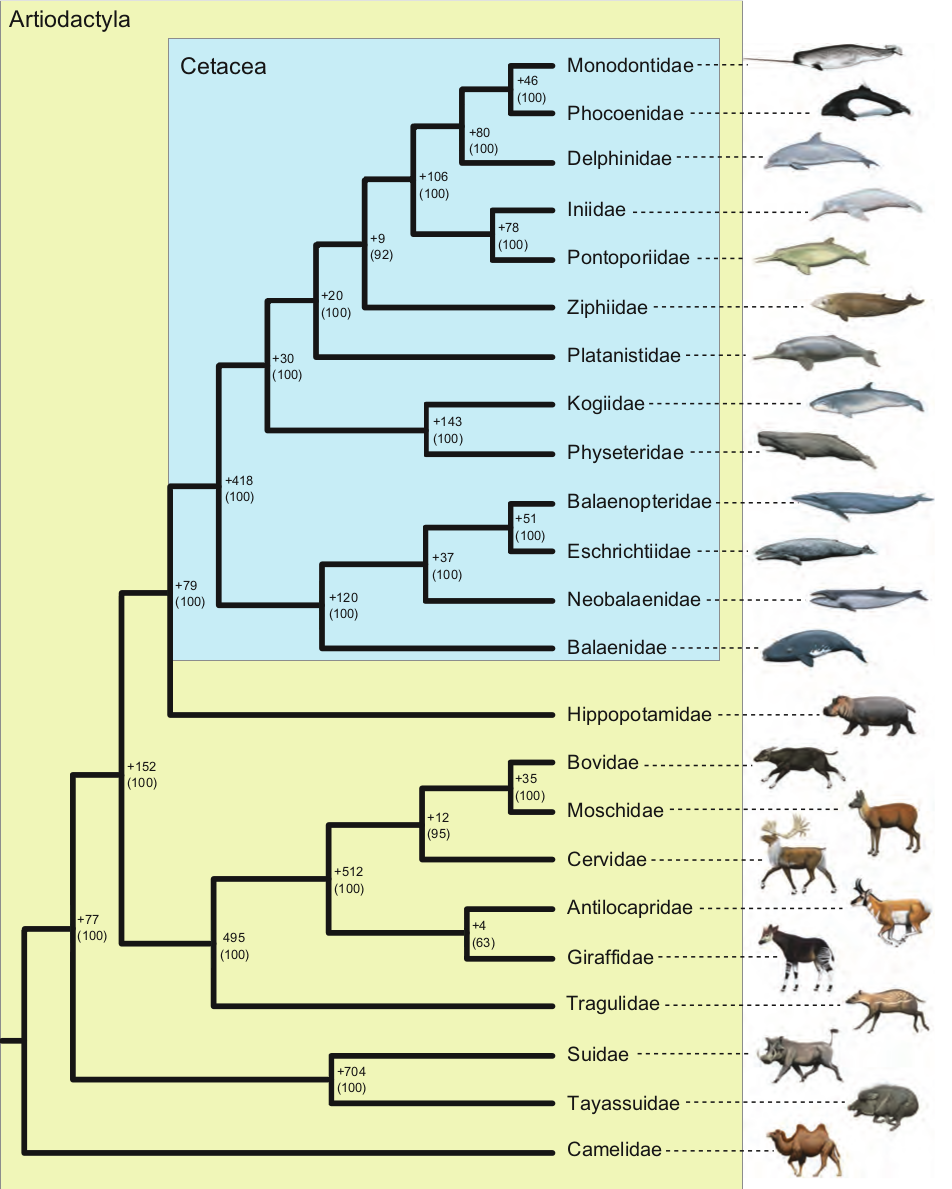
\includegraphics[width=0.5\linewidth]{figures/Gatesy_2012_phylogenetics_whale} 

}

\caption{\label{fig:tree01} The phylogenetic position of Cetacea relative to other extant artiodactyls. Bootstrap percentages are in parentheses to the right of nodes and below branch support scores. Modified from Gatesy, et al (2012).}\label{fig:unnamed-chunk-1}
\end{figure}
\begin{figure}

{\centering 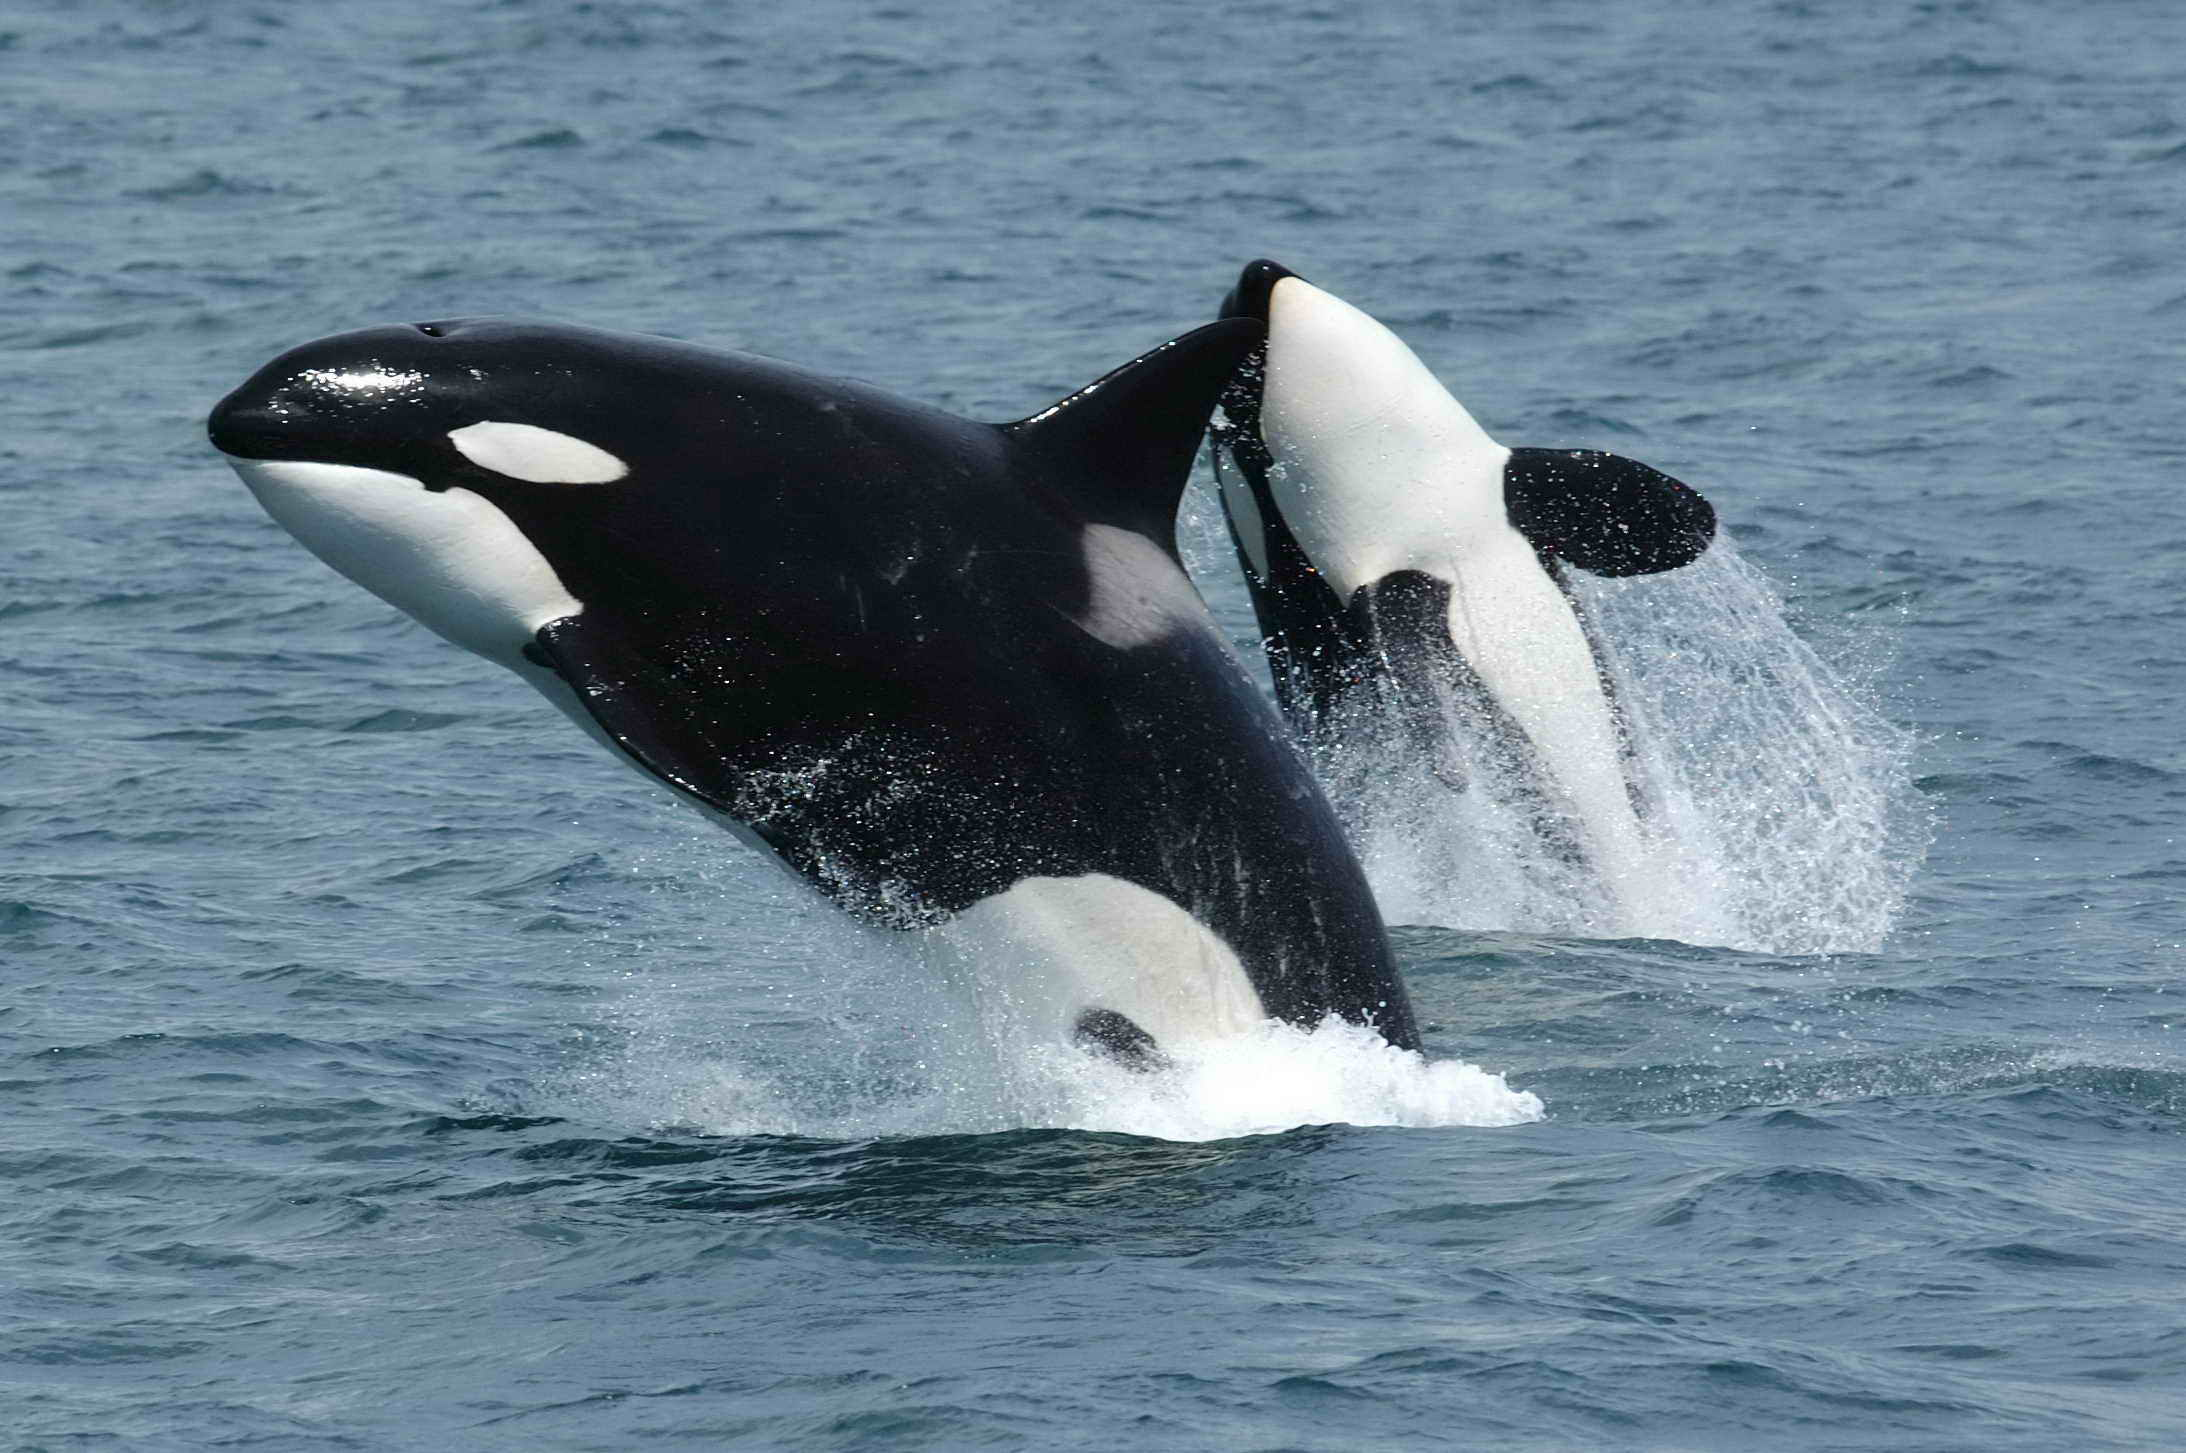
\includegraphics[width=0.8\linewidth]{figures/Killerwhales_jumping} 

}

\caption{\label{fig:photo_orca}Killer whales photographed off the south side of Unimak Island, eastern Aleutian Islands, Alaska. Photograph by Robert Pitman (NOAA).}\label{fig:unnamed-chunk-2}
\end{figure}

\hypertarget{methods}{%
\section{Methods}\label{methods}}

Recorded data of human sightings of all described cetacean species in
the delphinidae family corresponding to the period of 2010 to 2019 was
recollected from the Blobal Biodiversity Information Facility (GBIF).

This data was analyzed considering the species, genus, location and time
of each observation, and used to establish a global map of delphinidae
sightings during this last decade, to identify popular locations for
whale watching and to make predictions for the immediate future
regarding the expected number of sightings for the \emph{Orcinus orca}
species.

\hypertarget{results}{%
\section{Results}\label{results}}

\hypertarget{delphinidae-biodiversity}{%
\subsection{Delphinidae biodiversity}\label{delphinidae-biodiversity}}

\FloatBarrier

Human wildlife observations registered at GBIF from the start of 2010 to
2019/10/9, have produced 41956 observations of members of the
\emph{Delphinidae} family, registering global ocurrence data for 40
species, between 18 genera (Table \ref{table:species}).

\begin{table}
\caption{\label{tab:unnamed-chunk-3}\label{table:species} Observation data of members of the Delphinidae family obtained from the Global Biodiversity Information Facility, corresponding to the analysed period, depicting the number of occurrences per species. Species are grouped by genera utilising the same color palette used in all figures}

\centering
\begin{tabular}{l|l|r}
\hline
Genus & Species & Obs.\\
\hline
\em{Cephalorhynchus} & \em{commersonii} & 619\\
\hline
\em{Cephalorhynchus} & \em{eutropia} & 7\\
\hline
\em{Cephalorhynchus} & \em{heavisidii} & 8\\
\hline
\em{Cephalorhynchus} & \em{hectori} & 108\\
\hline
\em{Delphinus} & \em{capensis} & 208\\
\hline
\em{Delphinus} & \em{delphis} & 9017\\
\hline
\em{Feresa} & \em{attenuata} & 26\\
\hline
\em{Globicephala} & \em{macrorhynchus} & 409\\
\hline
\em{Globicephala} & \em{melaena} & 77\\
\hline
\em{Globicephala} & \em{melas} & 1224\\
\hline
\em{Grampus} & \em{griseus} & 1416\\
\hline
\em{Lagenodelphis} & \em{hosei} & 67\\
\hline
\em{Lagenorhynchus} & \em{acutus} & 711\\
\hline
\em{Lagenorhynchus} & \em{albirostris} & 537\\
\hline
\em{Lagenorhynchus} & \em{australis} & 171\\
\hline
\em{Lagenorhynchus} & \em{cruciger} & 67\\
\hline
\em{Lagenorhynchus} & \em{obliquidens} & 139\\
\hline
\em{Lagenorhynchus} & \em{obscurus} & 87\\
\hline
\em{Lissodelphis} & \em{borealis} & 35\\
\hline
\em{Lissodelphis} & \em{peronii} & 4\\
\hline
\end{tabular}
\centering
\begin{tabular}{r}
\hline

\hline
\end{tabular}
\centering
\begin{tabular}{l|l|r}
\hline
Genus & Species & Obs.\\
\hline
\em{Orcaella} & \em{brevirostris} & 11\\
\hline
\em{Orcaella} & \em{heinsohni} & 659\\
\hline
\em{Orcinus} & \em{orca} & 1880\\
\hline
\em{Peponocephala} & \em{electra} & 42\\
\hline
\em{Pseudorca} & \em{crassidens} & 211\\
\hline
\em{Sotalia} & \em{fluviatilis} & 35\\
\hline
\em{Sotalia} & \em{guianensis} & 69\\
\hline
\em{Sousa} & \em{chinensis} & 34\\
\hline
\em{Sousa} & \em{plumbea} & 6\\
\hline
\em{Sousa} & \em{sahulensis} & 1294\\
\hline
\em{Sousa} & \em{teuszii} & 4\\
\hline
\em{Stenella} & \em{attenuata} & 399\\
\hline
\em{Stenella} & \em{clymene} & 8\\
\hline
\em{Stenella} & \em{coeruleoalba} & 1578\\
\hline
\em{Stenella} & \em{frontalis} & 2217\\
\hline
\em{Stenella} & \em{longirostris} & 1207\\
\hline
\em{Steno} & \em{bredanensis} & 113\\
\hline
\em{Tursiops} & \em{aduncus} & 1188\\
\hline
\em{Tursiops} & \em{australis} & 5\\
\hline
\em{Tursiops} & \em{truncatus} & 13771\\
\hline
\end{tabular}
\end{table}

\hypertarget{sightings-per-country}{%
\subsection{Sightings per country}\label{sightings-per-country}}

\begin{figure}

{\centering 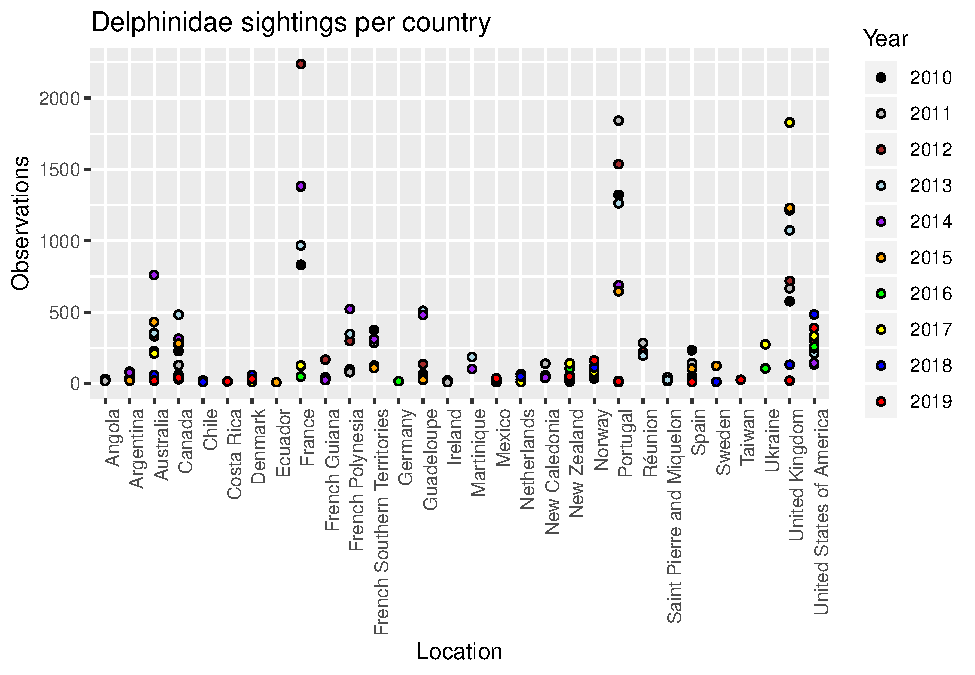
\includegraphics[width=1\linewidth]{SubjectEvaluation_3R_article_files/figure-latex/unnamed-chunk-4-1} 

}

\caption{\label{fig:plot_country_obs} Annual observation data during the analyzed period, countries with less than 10 recorded sighting events in a year were excluded.}\label{fig:unnamed-chunk-4}
\end{figure}

Utilizing GBIF data, the total \emph{Delphnidae} sightings during the
analized period were extracted and presented in figure
\ref{fig:plot_country_obs}. The country with most average sightings per
year was the United Kingdom, averaging 1032 yearly sightings. `

\hypertarget{diversity-per-country}{%
\subsection{Diversity per country}\label{diversity-per-country}}

\begin{table}
\caption{\label{tab:unnamed-chunk-5}\label{table:country_div} Delphinidae family biodiversity data per country. Table data includes countries with a biodiversity of at least 5 different species.}

\centering
\begin{tabular}{l|r}
\hline
Country & Biodiversity\\
\hline
Argentina & 5\\
\hline
Australia & 10\\
\hline
Canada & 9\\
\hline
France & 7\\
\hline
French Guiana & 7\\
\hline
Guadeloupe & 6\\
\hline
Mexico & 5\\
\hline
\end{tabular}
\centering
\begin{tabular}{r}
\hline

\hline
\end{tabular}
\centering
\begin{tabular}{l|r}
\hline
Country & Biodiversity\\
\hline
Netherlands & 5\\
\hline
New Zealand & 6\\
\hline
Norway & 6\\
\hline
Portugal & 8\\
\hline
Spain & 6\\
\hline
United Kingdom & 8\\
\hline
United States of America & 13\\
\hline
\end{tabular}
\end{table}

Only 41 countries had stable sightings of \emph{Delphinidae} species
(averaging more than one sighting per species, per year, during the
2010-2019period), from a total of 113 analyzed countries. The country
with the highest biodiversity was the United States of America, with 13
different species sighted during the period. Only 14 countries had more
than 5 different species observed during the period (Table
\ref{table:country_div}). Similarly 15 countries had minimal
biodiversity, at only 1 species with stable sightings.

\hypertarget{orcinus-orca-sightings-per-country}{%
\subsection{Orcinus orca sightings per
country}\label{orcinus-orca-sightings-per-country}}

\begin{figure}
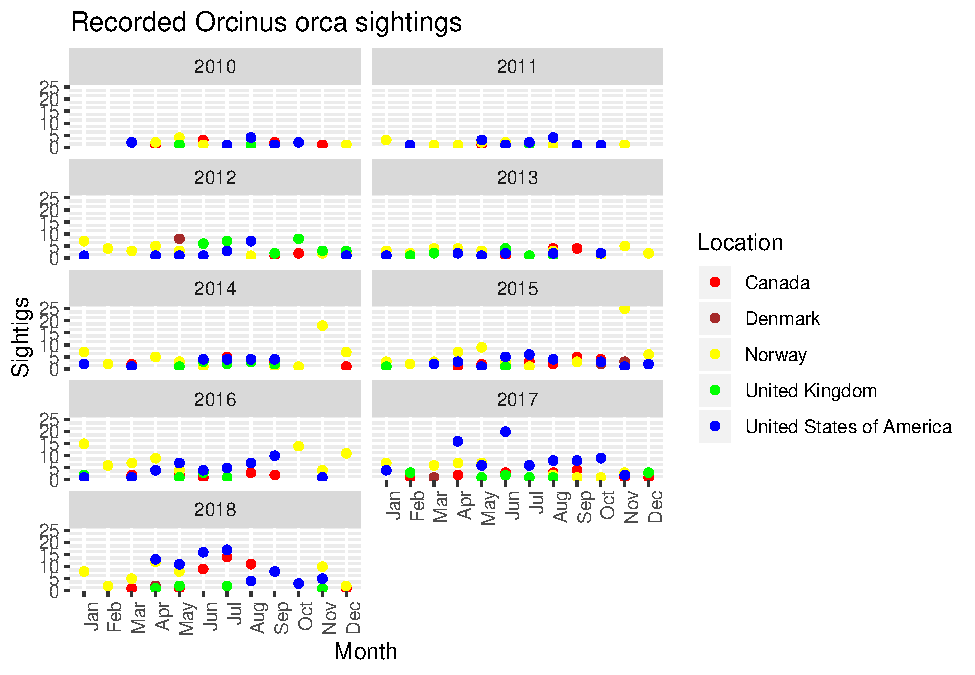
\includegraphics[width=1\linewidth]{SubjectEvaluation_3R_article_files/figure-latex/unnamed-chunk-6-1} \caption{\label{fig:orca_country} Yearly orca sightings from 2010 to 2018, in the countries with most stable sightings.}\label{fig:unnamed-chunk-6}
\end{figure}

Of the recorded species, perhaps none has had such a dramatic shift in
public perception as \emph{Orcinus orca}, initially considered dangerous
savage animals and even pests, whose populations were often actively
killed by both fishermen and governments due to their impact in fishing
and whaling activities. Even their name points to a sinister origin,
considering its common name of killer whale, and that \emph{orcinus}
from latin meaning, belonging to Orcus, the roman god of the
netherworld. Society's opinion on the animals began to change during the
late sixties, with the live capture of Moby Doll, and Bigg's researching
their complex social structures and the actual numbers of their heavily
reduced populations due to extensive ``hunting''. Unlike the most common
popular species, like \emph{Tursiops truncatus}, with 1530 yearly
sightings, orcas only average 209 sightings. Countries with the highest
stable sighting data for \emph{Orcinus orca} have had their yearly
recordings analyzed in figure \ref{fig:orca_country}.

\hypertarget{expected-sightings-in-the-near-future}{%
\subsection{Expected sightings in the near
future}\label{expected-sightings-in-the-near-future}}

\begin{table}[t]

\caption{\label{tab:unnamed-chunk-7}\label{table:model_fits} Tested predictive models using the data corresponding to the most diverse locations with the highest number of stable observations across the decade.}
\centering
\begin{tabular}{l|r|r}
\hline
Model & AIC & BIC\\
\hline
Year*Country & 1328.294 & 1367.248\\
\hline
Year+Month*Country & 1359.637 & 1554.406\\
\hline
Year*Month*Country & 1362.857 & 1709.901\\
\hline
\end{tabular}
\end{table}

\begin{figure}
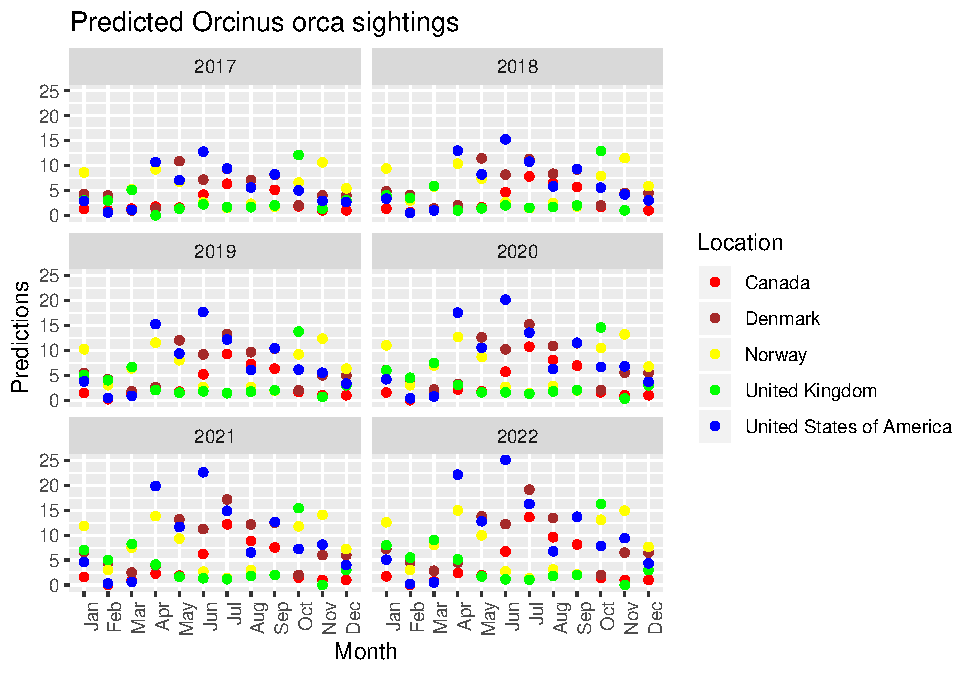
\includegraphics[width=1\linewidth]{SubjectEvaluation_3R_article_files/figure-latex/unnamed-chunk-8-1} \caption{\label{fig:plot_model_pred} Predicted orca sightings for the period of 2017 to 2022, for the analyzed countries.}\label{fig:unnamed-chunk-8}
\end{figure}

Using yearly sighting data obtained during this decade 3 predictive
models were constructed (Table \ref{table:model_fits}). Utilizing the
best fitted model predictions were made for the last 3 years and until
2022, regarding the expected orca sightings, per month for each of the
countries considered for the model (Figure \ref{fig:plot_model_pred}).

\FloatBarrier

\hypertarget{discussion}{%
\section{Discussion}\label{discussion}}

It is interesting to note that, as shown in
fig.\ref{fig:plot_model_pred}, most sightings tend to occur during the
summer months, so perhaps the quantity of recorded sightings, on a
specific month, might not be representative of the migratory behaviour
of these animals, and instead be dependant on the number of people
capable of taking such recordings and submitting them, a number that
would be expected to increase during summer vacations, explaining the
results.

Additionally, it is important to mention an outlier that had to be
excluded from the model, despite having some of the largest amount
records, 567 to be exact recorded during the 2010 to 2019 period,
however 563 observations up to 2013, only averaging 0.6 sightings per
year during the rest of the period, the reasons for this sudden
dissapearence of the species from the French Southern Territories is not
apparent, and would require further research to better understand it.

Finally, according to predicted data, the best month to observe orcas in
the wild is July, and the best location would be in the US, specifically
in Alaska.

\hypertarget{references}{%
\section*{References}\label{references}}
\addcontentsline{toc}{section}{References}

\hypertarget{refs}{}
\leavevmode\hypertarget{ref-perrin2009encyclopedia}{}%
1. Hoyt E. Whale watching, encyclopedia of marine mammals. Perrin WF,
Würsig B, Thewissen J, editors. Academic Press; 2009. pp. 1219--1223.

\leavevmode\hypertarget{ref-hoyt2001whale}{}%
2. Hoyt E, others. Whale watching 2001: Worldwide tourism numbers,
expenditures, and expanding socioeconomic benefits. Yarmouth Port, MA
(USA) IFAW; 2001;

\leavevmode\hypertarget{ref-gatesy2013phylogenetic}{}%
3. Gatesy J, Geisler JH, Chang J, Buell C, Berta A, Meredith RW, et al.
A phylogenetic blueprint for a modern whale. Molecular phylogenetics and
evolution. Elsevier; 2013;66: 479--506.

\nolinenumbers


\end{document}

